Una vez fijados los objetivos a abordar, en este capítulo se va a
describir la infraestructura concreta en la que nos hemos apoyado
para desarrollar las soluciones, tanto hardware como software.

\section{3DR Solo Drone}
Para este Trabajo Fin de Grado se ha elegido el dron 3DR Solo distribuido por la empresa norteamericana 3DRobotics \cite{3dr}\footnote{\url{https://3dr.com/}}. Este dron se encuentra en una gama alta debido a sus capacidades \footnote{\url{https://3dr.com/solo-drone/specs/}}, tales como batería, distancia de comunicacion y potencia, cualidades que lo hacen un dron muy versatil. Durante el desarrollo se ha usado la versión oficial del firmware de 3DR 2.4.2. Se eligió esa debido a que era una versión estable. A bordo de este dron se encuentra una placa estabilizadora Pixhawk 2.

Este drone incluye una tarjeta ArduIMU\footnote{\url{https://3dr.com/support/articles/arduimu_v3_kit/}}, es una Unidad de Medida Inercial (IMU) que integra un procesador compatible con Arduino y es capaz de ejecutar Attitude Heading Reference System (AHRS), basado en el algoritmo DCM (Direct Cosine Matrix) de Bill Premerlani. La tarjeta IMU consta de un acelerómetro de 3 ejes y tres sensores giroscópicos, un regulador de tensión dual (3.3V y 5V), un puerto de GPS, un Atmega328 @ 16MHz (como el Arduino Duemilanova), 3 LEDs de estado, cuenta con una MPU-6000 que integra un giroscopio que se comunica mediante el bus SPI, un magnetómetro HMC-5883L conectado mediante I2C y un Arduino Atmega328 de 16Mhz. La ArduIMU de la figura \ref{fig:arduimu} no es ninguna placa de navegación o piloto automático, sólo una placa de orientación y se puede utilizar en cualquier dispositivo del cual deseemos conocer su orientación con respecto al suelo – barcos, coches, aviones.

\begin{figure}[H]
  \centering
  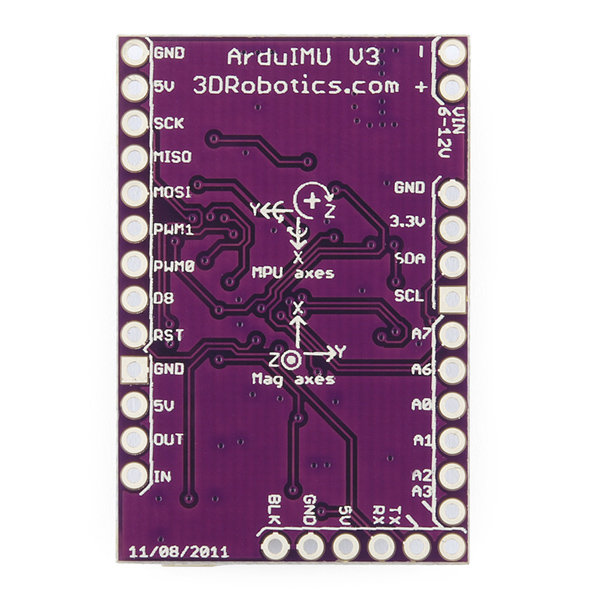
\includegraphics[scale=1]{imagenes/arduimutrasera.jpg}
  \caption{ArduIMU}
  \label{fig:arduimu}
\end{figure}

El mando del Solo drone proporciona los mecanismos de control y muestra los datos del vuelo en una pantalla a todo color. Mediante el uso de antenas dobles de largo alcance, el mando actúa como el eje central para todas la comunicaciones de la red Link 3DR via radio, recibe todas las comunicaciones de Solo y la aplicación de tierra, reenvía las salidas telemétricas a la aplicación y administra la transmisión de todas las entradas de control a Solo.

\begin{figure}[H]
  \centering
  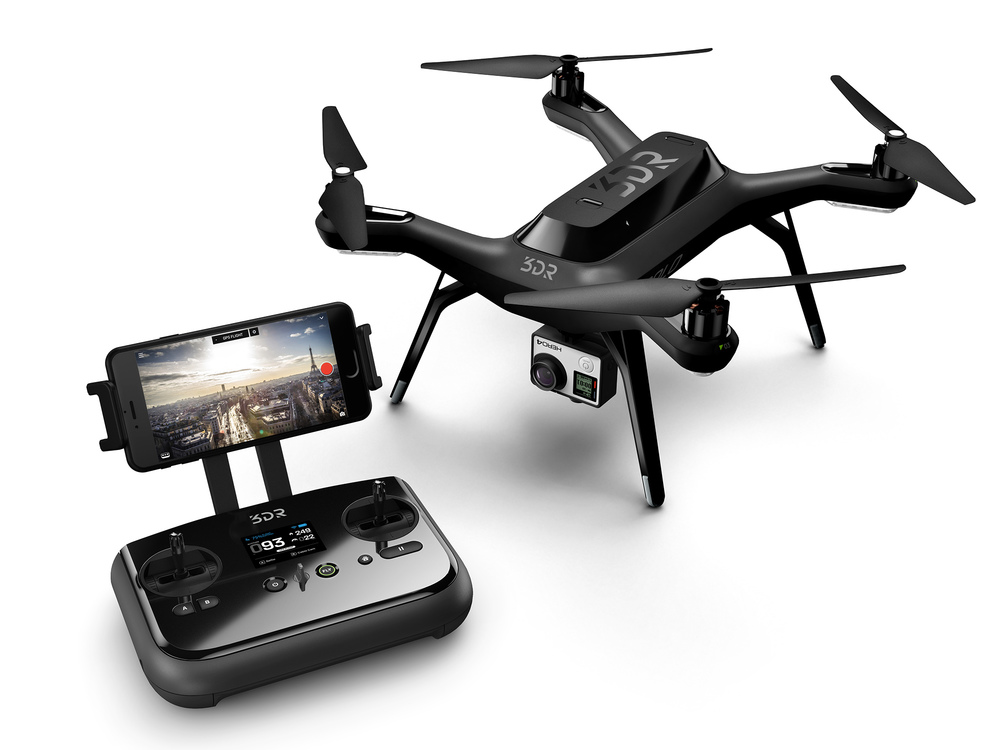
\includegraphics[scale=1]{imagenes/3drSoloDron.jpg}
  \caption{3DR Solo Drone}
  \label{fig:3drsolodrone}
\end{figure}

El único modo de conectar con el 3DR Solo será a través del mando, debido a que únicamente él es capaz de levantar la red wifi a la que conectarse. En posteriores evoluciones tanto del dron como del mando, desde los foros oficiales de 3DR \footnote{\url{https://3drpilots.com/threads/connecting-directly-to-the-pixhawk-2-on-a-solo.7926/}}. Comentan que ya se aborda la solución de que sea el propio dron quien levante la red wifi a la cual conectar y no tener que depender del enlace del mando.

Este dron incluye una placa estabilizadora Pixhawk. Esta placa es un desarrollo específico creado por la ``Pixhawk\cite{pixhawk} open hardware community" en colaboración con 3D Robotics y que vio como primer destinatario el 3DR Solo. Ofrece un interfaz que se apoya en el protocolo MAVLink. A través de estos comandos se le puede también enviar órdenes al piloto automático. 

\section{Protocolo MAVLink}
\label{sec:mavlink}

MAVLink\cite{mavlink} (Micro Air Vehicle Link) es un protocolo desarrollado para comunicar las placas estabilizadoras dotadas de piloto automático a los GCS (\textit{Ground Control Station}) o estación de tierra con las aplicaciones desde las que se envía misiones y se monitoriza el cumplimiento de las mismas desde tierra.
MAVLink se publicó \footnote{\url{https://github.com/mavlink/mavlink/commit/a087528b8146ddad17e9f39c1dd0c1353e5991d5}} en 2009 por Lorenz Meier, con licencia LGPL. Aspira a convertirse en el protocolo standard en robótica aérea y se ha probado su funcionamiento en PX4, PIXHAWK, APM\footnote{Ardupilot Mega} y Parrot AR.Drone.

La lista completa de los comandos de este protocolo se encuentra en la pagina oficial de Mavlink\footnote{\url{http://mavlink.org/messages/common}}. La versión actual que se está utilizando en este TFG es la 2.0. 

Cada comando tiene un identificador único  el cual permite al dron reconocer la acción que se debe realizar. En función de este identificador los parámetros que se introducen a continuación dan la información necesaria al dron para actuar. Un ejemplo de la estructura del mensaje que se usa para GPS es el siguiente:
\begin{lstlisting}[frame=single]
type GpsStatus struct {
    SatellitesVisible  uint8      
    SatellitePrn       [20]uint8  
    SatelliteUsed      [20]uint8  
    SatelliteElevation [20]uint8  
    SatelliteAzimuth   [20]uint8  
    SatelliteSnr       [20]uint8  
}
\end{lstlisting}
Este mensaje trae la información del enlace actual con el GPS y se envía periódicamente en ciclos cuya frecuencia se configura en los parámetros de conexión con el dispositivo.

Un ejemplo de los mensajes más importantes del protocolo en los que se centra este TFG es el comando de velocidad. Este comando hace uso de la estructura del mensaje ``SET\_POSITION\_ TARGET\_LOCAL\_NED'', en el cual se indican las velocidades lineales que debe seguir en cada eje (en m/s). Este comando, junto con el de ordenar la rotación, cuya estructura es la del mensaje "COMMAND\_LONG", permite tener control total sobre las velocidade del dron. 

En la figura \ref{fig:comunicacionMAVLink} se puede comprobar la estructura de la comunicación entre la estación de tierra y cada componente se establece. Continuamente se intercambian mensajes con información, ya sea para comunicar una acción, reclamar el estado de algún componente interno, como podría ser la batería, o un simple ACK para mantener la conexión activa.


\begin{figure}[H]
  \centering
  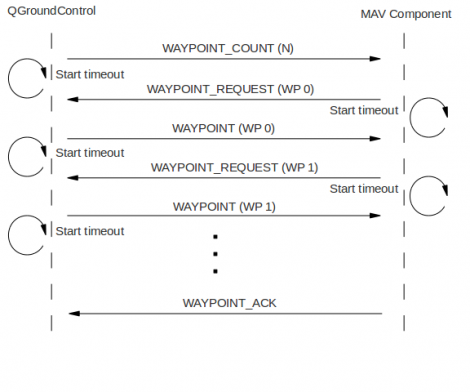
\includegraphics[scale=0.5]{imagenes/comunicacionMavLink.png}
  \caption{Comunicación MAVLink}
  \label{fig:comunicacionMAVLink}
\end{figure}

\subsection{Software MavProxy}
\label{sec:MavProxy}

MavProxy\cite{mavproxy} es un módulo controlador multihilo que simplifica el uso del protocolo MAVLink desde aplicaciones en Python. Es un GCS totalmente funcional (sistema de comunicación grupal) para UAV, la versión 1.4.38 es utilizado en este trabajo fin de grado. Es un GCS minimalista, portátil y extensible para cualquier UAV que soporte el protocolo MAVLink. Tiene una serie de características clave, que incluyen la capacidad de reenviar mensajes de UAV a través de UDP (User Datagram Protocol) a otros programas de estación terrestre en otros dispositivos. Una de las opciones más interesantes de MAVProxy es que permite reenviar mensajes provenientes de nuestro UAV hacia diferentes GCS ubicadas en diversas plataformas como ordenadores, tabletas o teléfonos móviles. De la misma manera, podemos enviar comandos en tiempo real al UAV desde el GCS\cite{danielPlaza}.

\begin{figure}[H]
  \centering
  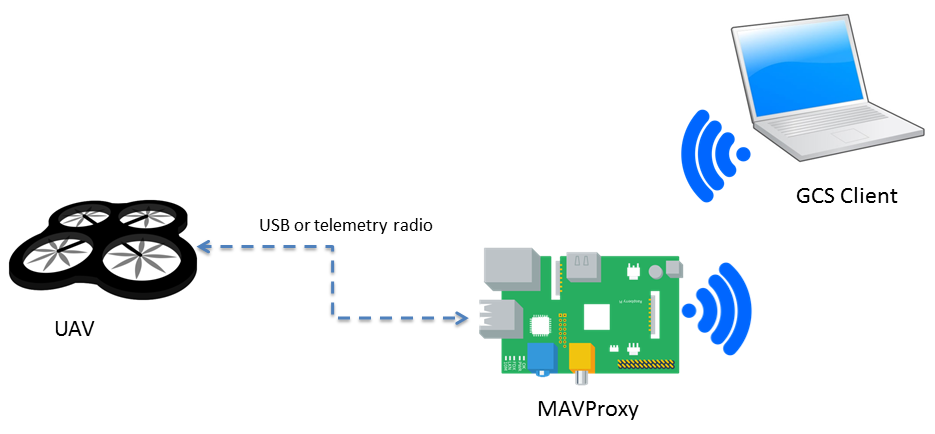
\includegraphics[scale=0.4]{imagenes/bridge.png}
  \caption{MavProxy}
  \label{fig:mavProxy}
\end{figure}

MAVProxy permite ordenar el diálogo desde un programa en Python con un UAV a través de varios canales simultáneos. Simplifica tanto la lectura de mensajes del UAV, típico de la información sensorial, como el envío de mensajes al UAV, típico de las órdenes de actuación (tanto de comandos de velocidad como puntos de paso para las misiones). Además también simplifica el intercambio de mensajes de configuración.

Tiene como principales características:

\begin{itemize}
\item Es una aplicación de línea de comandos y consola. Hay complementos incluidos en MAVProxy
para proporcionar una GUI básica.
\item Está escrito en Python.
\item Es de código abierto.
\item Es portátil; debería ejecutarse en cualquier sistema operativo POSIX con Python, pyserial y función
llamadas, lo que significa Linux, OS X, Windows y otros.
\item Admite módulos cargables y tiene módulos para admitir consolas, mapas en movimiento,
joysticks, seguidores de antena, etc.
\end{itemize}

\section{JdeRobot}
\label{sec:jderobot}

JdeRobot\cite{jderobot} es un entorno desarrollado por el laboratorio de robótica de la Universidad Rey Juan Carlos para el desarrollo de aplicaciones de robótica. Su última versión la 5.6 \footnote{\url{https://github.com/JdeRobot/JdeRobot}} se liberó el 9 de Octubre de 2017 y es la usada en este TFG. JdeRobot se compone de interfaces, drivers, utilidades y aplicaciones para el desarrollo de proyectos de robótica. Las aplicaciones y los drivers se comunican intercambiando mensajes entre sí utilizando interfaces ICE o interfaces ROS.

Algunos de los drivers más importantes que contiene:
\begin{enumerate}
\item Cameraserver. Para enviar imágenes y video a través del interfaz ICE camera.
\item Gazeboserver. Conjunto de plugins en el simulador Gazebo que ejercen de drivers entre las aplicaciones inteligentes y los robots simulados.
\item Ardrone\_server. Driver que ofrece acceso a los sensores y actuadores del Parrot Ar-Drone a través de interfaces ICE \footnote{\url{http://jderobot.org/Amartinflorido-tfg}}. Está escrito en C++, transforma el conjunto de comandos AT del drone en interfaces y viceversa, implementa los interfaces camera, cmdvel, navdata, extra y pose3D y permite acceder a la actitud del drone así como a sus 2 cámaras. Sirve también datos como el nivel de la batería y permite grabar vídeo o tomar fotos.
\end{enumerate}
Algunas de las herramientas disponibles en JdeRobot más usadas en este TFG son:
\begin{enumerate}
\item Cameraview. Una aplicación desarrollada en C++ capaz de recibir vídeo a través del interfaz camera.
\item UAV viewer. Aplicación desarrollada como control en tierra de robots aéreos. Permite teleoperar cualquier tipo de robot aéreo utilizando interfaces ICE. Ofrece de forma visualmente atractiva datos como la actitud, velocidades lineales y angulares, ofrece también la posibilidad de visualizar videos servidos por el interfaz camera como se ve en la figura \ref{fig:uav_viewer_old} \footnote{\url{http://jderobot.org/Amartinflorido-tfg}}. Existen varias versiónes de esta aplicación, escritas en lenguajes como C++, Javascript y la desarrollada en este Trabajo Fin de Grado en Python. Ofrece información del drone en tiempo real de los parámetros de vuelo como pueden ser la posición o velocidad. También permite teleoperar el drone mediante comandos de velocidad y ordenes de aterrizaje o despegue.

\begin{figure}[H]
  \centering
  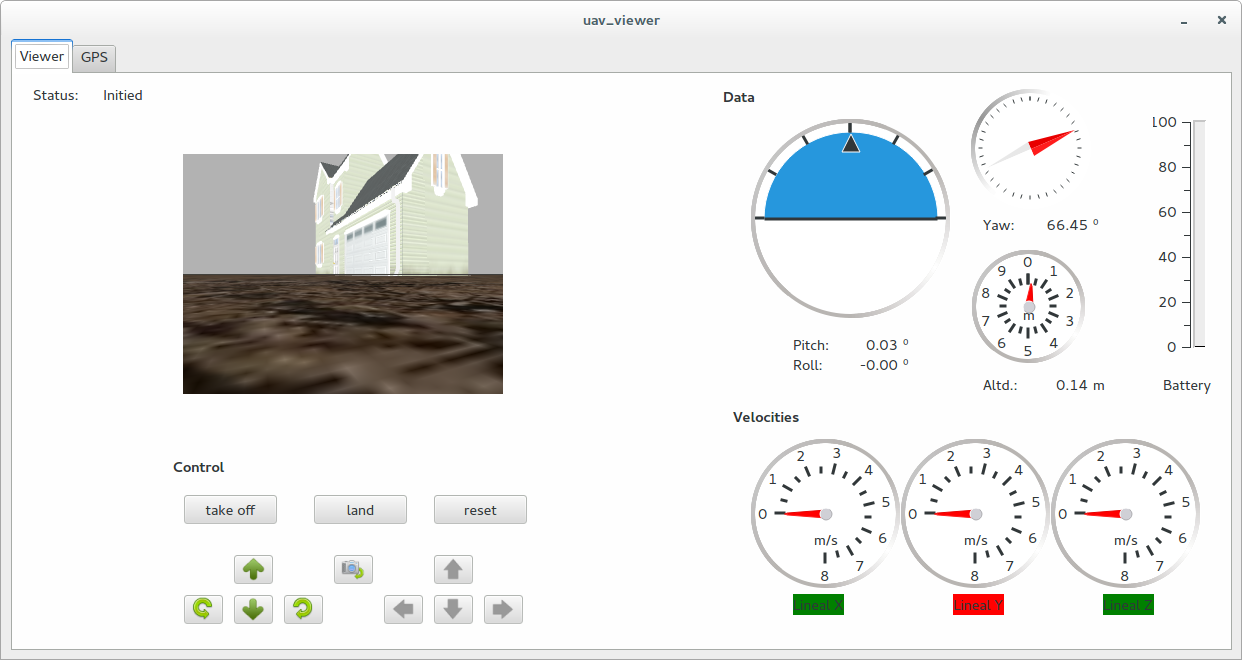
\includegraphics[scale=0.2]{imagenes/uav_viewer_old.png}
  \caption{UAV Viewer}
  \label{fig:uav_viewer_old}
\end{figure}
\end{enumerate}

\subsection{Interfaces ICE relativos a los drones}
JdeRobot dispone de más de 30 interfaces pero los que se han utilizado durante este TFG que son los relacionados con los drones, son:
\begin{itemize}
\item Pose3D. Recoge los datos de actitud y la posici\'on tridimensional de la aeronave. La posición se expresa como coordenadas cartesianas absolutas respecto de cierto sistema de referencia arbitrario
y el ángulo se expresa en forma de cuaternión. 

\begin{lstlisting}[frame=single]
Pose3DData
  {
	float x;  /* x coord */
	float y;  /* y coord */
	float z;  /* z coord */
  	float h;  /* */
	float q0; /* qw */
	float q1; /* qx */
	float q2; /* qy */
	float q3; /* qz */
  };
\end{lstlisting}

\item CMDVel. Utilizado para enviar comandos de velocidad. Las variables ``linear'' afectan a la velocidad de traslacion relativa del drone, es decir, al avance o retroceso (linearX), al desplazamiento lateral (linearY) o al ascenso y descenso (linearZ). Por otro lado las variables ``angular'' se corresponden a las velocidades angulares, guiñada (angularX), alabeo (angularY) o cabeceo (angularZ). 
\begin{lstlisting}[frame=single]
	class CMDVelData
	{
		float linearX;
		float linearY;
		float linearZ;
		float angularX;
		float angularY;
		float angularZ;										
	};
\end{lstlisting}
\item Extra. Utilizado principalmente para las órdenes de despegue y aterrizaje.
\begin{lstlisting}[frame=single]
    void land() - land drone. 
    void takeoff() - takeoff drone. 
    void reset() 
    void recordOnUsb(bool record) 
    void ledAnimation(int type,float duration, float req) 
    void flightAnimation(int type, float duration) 
    void flatTrim() 
    void toggleCam() - switch camera. 
\end{lstlisting}

\end{itemize}

\clearpage
\subsection{COMM}
Biblioteca de mensajes que se sitúa entre las aplicaciones y los interfaces de comunicacion, ICE o ROS. Esta biblioteca se ha desarrollado recientemente en JdeRobot como mediador entre las aplicaciones para comunicar indistintamente todos los drivers con la finalidad de abstraer del tipo de comunicación que se realice.

\section{Biblioteca de comunicaciones ICE}
\label{sec:ICE}
ICE\footnote{\url{https://zeroc.com/products/ice}}\cite{ice} (Internet Communications Engine) es un \textit{middleware}  orientado a objetos que proporciona llamadas a procedimientos remotos, \textit{grid computing} y funcionalidad cliente / servidor desarrollada por ZeroC con una licencia GNU GPL y también una licencia privativa. ICE trabaja con objetos distribuidos, pueden estar en diferentes máquinas y comunicarse a través de la red a enviándose mensajes entre ellos. 

ICE permite desarrollar aplicaciones distribuidas con un esfuerzo mínimo, abstraer al programador para que interactúe con una red de manera simple, usando interaces entre objetos distribuidos. El desarrollo de aplicaciones se enfoca así sólo en la lógica y no en las peculiaridades de la red. Es un \textit{middleware} multilenguaje, podemos implementar clientes y servidores en diferentes lenguajes de programación y en diferentes plataformas. Está disponible para C++, Java, .Net languages, Objective-C, Python, PHP y Ruby, en la mayoría de los sistemas operativos. También hay una versión para teléfonos móviles llamada Ice-e. 

JdeRobot puede utilizar ICE para la comunicación entre sus nodos, por lo tanto, la tarea de leer
los valores de un sensor u órdenes de comando a un robot son tan simples como ejecutar un método de un objeto en la aplicación. Una ventaja significativa es la posibilidad de desarrollar aplicaciones independientes del contexto. Un programador puede desarrollar un driver en C++ para un robot particular que está incrustado en el robot, por otro lado, otro desarrollador puede programar una aplicación para el procesamiento de imágenes en Python que se ejecuta en un PC. Mediante ICE se pueden usar estas dos piezas, que originalmente eran independientes, como una sola aplicación sin preocuparse por las comunicaciones de bajo nivel.

La conexión entre el driver desarrollado en este TFG y las aplicaciones de control, así como la propia herramienta de teleoperación, se han realizado usando este \textit{middleware}.

\clearpage
\section{Python}
\label{sec:python}

Python\cite{python} es un lenguaje de programaci\'on interpretado y multiplataforma que naci\'o en los años 80 con idea de hacer más legible el c\'odigo.
Inicialmente se utilizaba para scripting, ha sabido crecer con los años y con la publicaci\'on de Python3 en 2009 ha recibido el impulso que necesitaba para ser hoy en día el 5º lenguaje más utilizado, por encima de PHP, .NET y Javascript, que baja hasta el 8º puesto según TIOBE en un estudio de Abril de 2017.

Tanto el driver como la herramienta desarrollados en este TFG se han creado empleando Python 2.7. El empleo de esta versión se debe a que JdeRobot es compatible con ROS y este \textit{framework} únicamente es compatible en dicha versión de Python. Los motivos de utilizar Python son varios: mantiene el carácter multiplataforma de JdeRobot, su c\'odigo es simple y legible y trabaja bien con dependencias muy utilizadas en rob\'otica como OpenCV.


\cleardoublepage